\chapter{Network Types and Solutions Proposed}
\label{cha:netsolutions}
As mentioned earlier in this dissertation, optimal solutions have high computational cost whilst the algorithms proposed in this work can be applied to large scale networks; when working with these kind of solutions it is not possible to exactly know which node is going to contribute best to the influence spread. However, full network knowledge is still given and it is possible to use it to extract the basic features that characterize that network, and therefore estimate the expected diffusion value of a node based on its properties and role in the network. The proposed solutions consider the following aspects when deciding the best nodes to choose:
\begin{itemize}
\item Node Activity, based on the node's degree
\item Node Spread Paths, based on how wide is the reach of the cascade originated by every node
\item Node Activation, based on node reachability
\item Node Temporal Position, based on how much of the time window the node affects
\end{itemize}

Different strategies are proposed, some considering more activity based characteristic like node degree and some focusing more on the temporal aspects of the network, like node coverage and activation time. The goal is too measure the performance of those strategies on different networks, each of them varying in size, and edges' frequency and temporal distribution. After analyzing the results it is possible to see if non optimal solutions proposed under these realistic network and budget conditions can still produce a good influence spread, and compare which strategy works best under some specific network circumstance.

\section{Network Datasets}
\label{sec:data}
The strategies are evaluated on realistic temporal network Datasets all based on interactions between two people, presented here:
\begin{itemize}
\item Message Dataset (College) - 1899 nodes, 59835 edges, start time 1082040961, end time 1098777142, no simultaneous edges
\item Proximity Conversation Dataset (Ia) - 113 nodes, 20818 edges, start time 20, end time 212360, presence of simultaneous edges
\item Chat Dataset (SFHH) - 403 nodes, 70261 edges, start time 32520, end time 146820, presence of simultaneous edges
\end{itemize}

\section{Network Features}
\label{sec:necfeats}
Networks are always different from each other, because of the size and the number and concentration of the edges/users. However studies about small world properties \cite{https://doi.org/10.48550/arxiv.2103.08035} prove that seemingly random networks have some type of correlation. These facts are even more emphasized in temporal networks, because they can be interpreted as a sequence of static networks. This means that not only the size and the concentration of the network can vary but also the distribution of the edges over its time window. Networks can be roughly grouped following those key aspects:
\begin{itemize}
\item Highly/Lowly Connected Networks
\item Homogeneous/Heterogeneous Networks
\item Unreachable/Isolated Nodes Networks
\item Time Balanced/Unbalanced Networks
\end{itemize}

\subsection{Highly Connected Networks}
\label{sec:hynets}
These kind of Networks are characterized by a higher edges to nodes ratio; this means that the average number of outgoing edges per node in the network is higher. Notice how in our specific study scenario, with limited budget, this can not ensure us any preliminary expectation about any influence spread because we don't know how the average degree of the nodes is actually distributed, and with limited budget we could be able to select only the nodes with way below average degree.  
The Proximity Dataset and the Chat Dataset are good examples of that since they have an high edges to nodes ratio of well over 100: however they do differentiate in terms of the number of nodes, meaning that in the Ia Dataset there are more interactions that occur multiple times at different timestamps. 
\begin{center}
    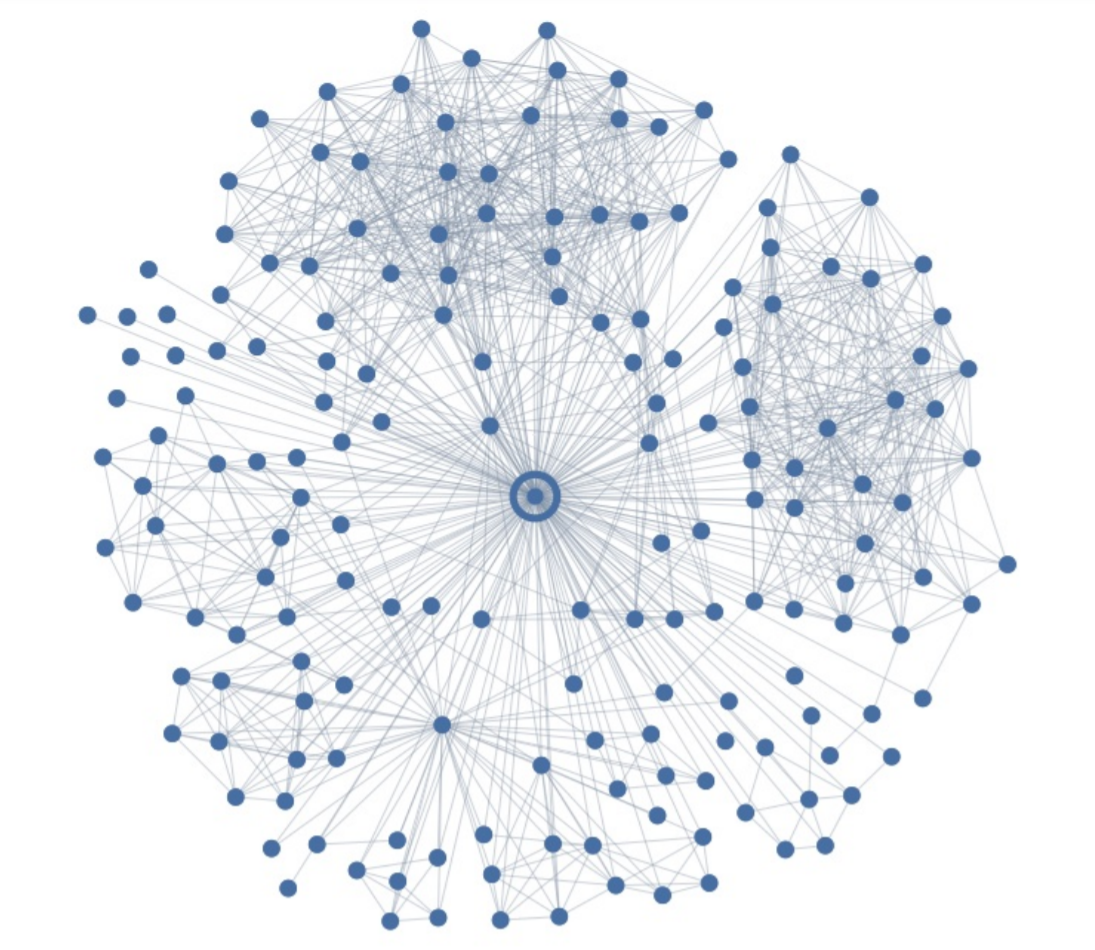
\includegraphics[scale=0.2]{highconets}
    \\
    Figure 4.1: Highly Connected Network Overview
\end{center}

\subsection{Lowly Connected Networks}
\label{sec:lownets}
These kind of Networks are characterized by a lower edges to nodes ratio: this means that the average number of outgoing edges per network node is lower. Generally we expect the worst influence spread in these kind of networks, because if there are few nodes with higher degree they are probabily going to be unaffordable, and on the other hand if the edges are distributed in a uniform way among the nodes, they are going to be very low in number.
\begin{center}
    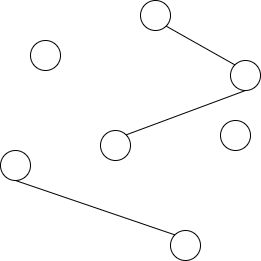
\includegraphics[scale=0.8]{lowconets}
    \\
    Figure 4.2: Lowly Connected Network Overview
\end{center}

\subsection{Unreachable/Isolated Nodes Networks}
\label{sec:isonets}
A node is said to be isolated when it has no edges pointing in and out of himself, hence both its in degree and out degree are zero. An unreachable node is a node whose in degree is still zero, however he has some edges pointing out of him and therefore can be useful to spread influence. This can be also common in lowly connected networks. In some networks with a higher number of unreachable nodes it might be worth to consider infecting some of them, other wise they are going to be cut out of the network forever.

\begin{center}
    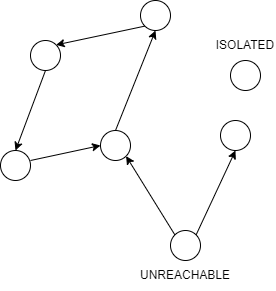
\includegraphics[scale=0.5]{isolated}
    \\
    Figure 4.3: Isolated/Unreachable Nodes Network Overview
\end{center}


\subsection{Time Balanced/Unbalanced Networks}
\label{sec:timenets}
Temporal Networks hide some problems related to node reachability: some nodes might be accessible only at certain times, and according to the network's temporal structure these times can be located earlier in the time window or later. The earlier those times are, the more difficult it is to reach a node, because there is less time for other interactions to happen that can generate a cascade leading to that node, whilst if a node can directly be accessed only at a later time step, there is more probability of other nodes activating earlier who can generate a cascade that includes that node. This obviously depends entirely on the network structure and the users interactions.
On top of that, time plays a key factor in the growth of the spreading curve. Different strategies that infect different nodes are going to develop differently, and given full network structure it is possible to make some observations and differentiate between nodes who can contribute a lot, and nodes that can contribute earlier and use as much time as possible. This is also enhanced by the fact that time is not related to the node cost in our modeled system, while degree is.

\begin{center}
    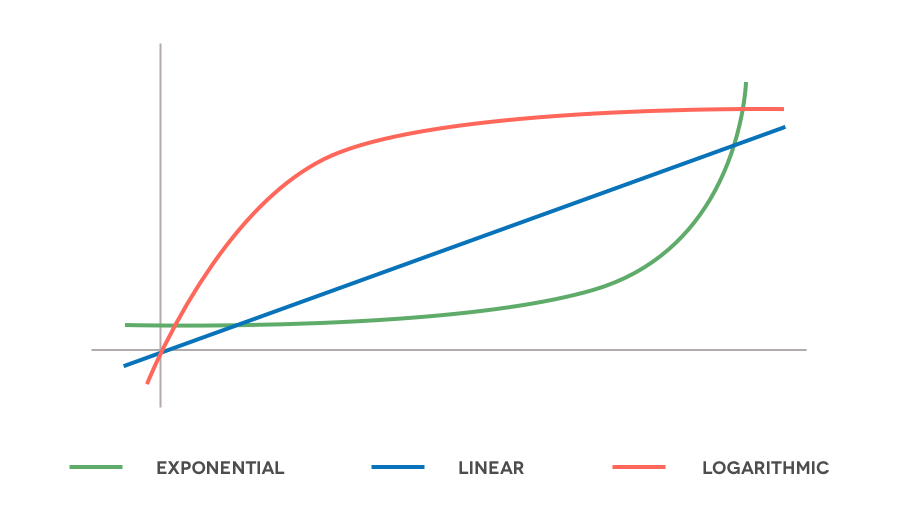
\includegraphics[scale=0.5]{curves}
    \\
    Figure 4.4: Different curves with different growth speed
\end{center}

\section{Influence Maximization Strategies}
\label{sec:strats}
In this section, we introduce the strategies implemented and studied. Each strategy is based on some possible network feature, with some of them being natural extension of static influence maximization strategies and some other strongly based on the temporal aspect of the network.
Each strategy was slightly optimized by not allowing to select two nodes with common neighbors. This enables an optimal usage of the budget along with good initial node coverage. What follows is a list of the strategies with a brief explaining of the idea behind the strategy, its code and how its characterized.

\subsection{Highest Degree Nodes (HDN)}
\label{sec:stratgreedy}
The idea behind this strategy is the simplest among all: we try to estimate the expected diffusion value of a node through its activity in the network, the more it interacts the more it can spread influence. It's greedy oriented and it is implemented to have a final clear report of how important it is to consider the time factor to estimate a node's expected diffusion value. Although this strategy might look pretty solid on the most basic influence maximization frameworks, there are some drawbacks:
\begin{itemize}
    \item Nodes with higher degree have higher cost, which means this strategy tends to build rather small seed sets
    \item Cost is not optimized. Given the exponential function to compute a node cost, picking a node with degree k costs more than picking two nodes each of them with degree k/2
    \item Temporal aspect is absolutely ignored. If the selected nodes interact only at the last time steps of the network almost every edge is wasted, resulting in poor performance
\end{itemize}

\begin{center}
    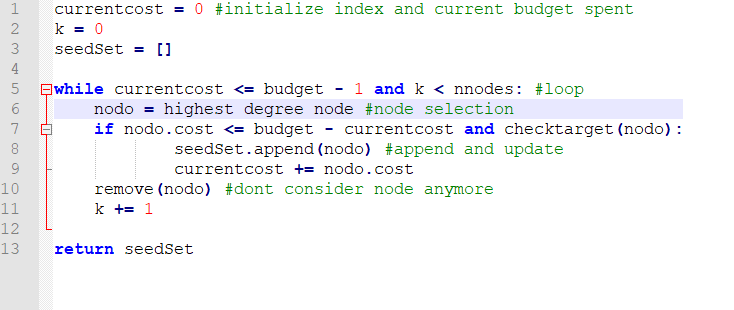
\includegraphics[scale=0.6]{/PseudoCode/greedy}
    \\
    Figure 4.5: Pseudo code For HDN function
\end{center}

\subsection{Highest Degree's Cheapest Neighbor (HDCN)}
\label{sec:stratneighbors}
This strategy is born after the main drawbacks of the First One. Here, the idea is to mitigate the cost, by trying to affect one of the neighbors of the highest degree node in order to try and save budget. This strategy ignores temporal aspects as well, as it just aims at seeding the cheapest among the neighbors, to secure more seed nodes given the fact that cheap nodes are more budget effective. 

\begin{center}
    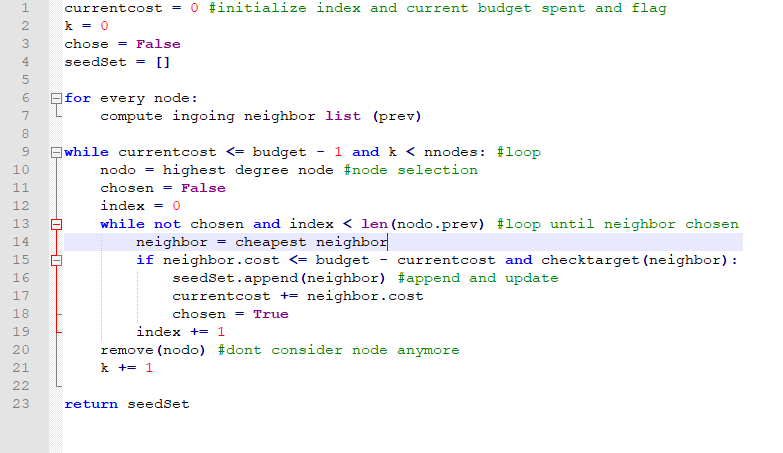
\includegraphics[scale=0.6]{/PseudoCode/neighbor}
    \\
    Figure 4.6: Pseudo code For HDCN function
\end{center}

\subsection{Earlier Nodes (EN)}
\label{sec:strattimeorder}
This strategy is purely based on the temporal aspect of the network. It also follows a greedy approach but adds the nodes that appear earlier in the network interactions, to maximize the influence and the time span used. The strategy does not take into account node degree at all (unless earlier nodes are tied in time), so the degree of the first nodes impact the strategy's overall performance.

\begin{center}
    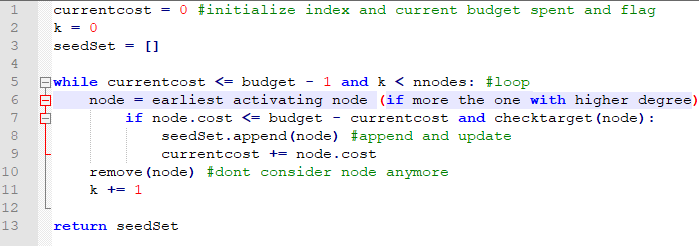
\includegraphics[scale=0.9]{/PseudoCode/early}
    \\
    Figure 4.7: Pseudo code For EN function
\end{center}

\subsection{Unreachable, Time Oriented Nodes (UTON)}
\label{sec:strattimeiso}
The idea behind this strategy is to take advantage of highly connected networks, where reachable nodes are well connected each other. The strategy aims at seeding the nodes that have less probability of being reached, with unreachable nodes (if any) being the first nodes to be seeded. When more unreachable nodes, the earliest to activate are taken first. This strategy allows to include nodes that would get easily cut out of the network, but does not consider node degree.

\begin{center}
    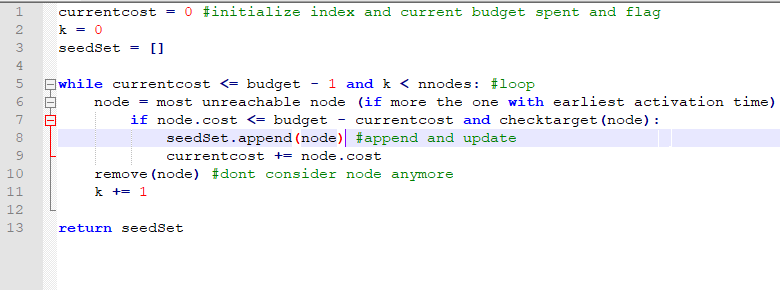
\includegraphics[scale=0.8]{/PseudoCode/unreachtime}
    \\
    Figure 4.8: Pseudo code For UTON function
\end{center}

\subsection{Unreachable, Degree Oriented Nodes (UDON)}
\label{sec:stratdegreeiso}
This strategy is a variant of the previous one, but here multiple unreachable nodes are taken first the higher their degree is.  This strategy allows to include nodes that would get easily cut out of the network, but relies more on a degree factor rather than a temporal one.

\begin{center}
    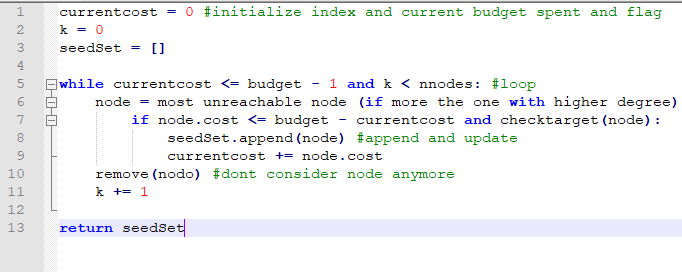
\includegraphics[scale=0.9]{/PseudoCode/unreachdeg}
    \\
    Figure 4.9: Pseudo code For UDON function
\end{center}

\subsection{Max Cover Nodes (MC)}
\label{sec:maxcover}
The final proposed strategy, as its name says, aims at maximizing the ideal cover of the influence spread. Based on a greedy approach and heavily relying on temporal aspects, this strategy adds one node at a time taking the node that can provide the most gain in terms of nodes reached by the seed set. This means that the ideal result of this strategy is always the best with any network structure, but the Probability Pspread plays a crucial role in determining the actual performance of this strategy.

\begin{center}
    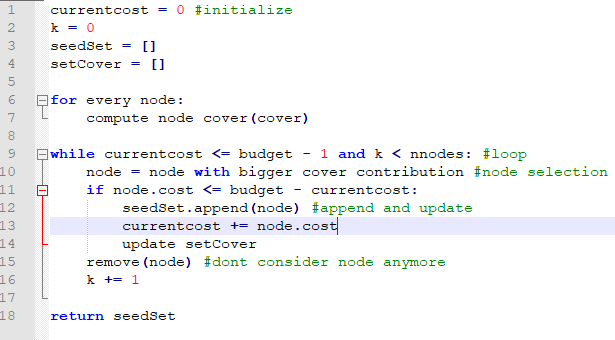
\includegraphics[scale=0.9]{/PseudoCode/maxcoverpseudo}
    \\
    Figure 4.10: Pseudo code For MC function
\end{center}
